%%%%%%%%%%%%%%%%%%%%%%%%%%%%%%%%%%%%%%%%%%%%%%%%%%%%%%%%%%%%%%%%%%%%%%%%%%%%%%%
\section{Possible Solutions}
%%%%%%%%%%%%%%%%%%%%%%%%%%%%%%%%%%%%%%%%%%%%%%%%%%%%%%%%%%%%%%%%%%%%%%%%%%%%%%%


%%%%%%%%%%%%%%%%%%%%%%%%%%%%%%%%%%%%%%%%%%%%%%%%%%%%%%%%%%%%%%%%%%%%%%%%%%%%%%%
\subsection{Angular Dependent Cross Section Implementations}
%%%%%%%%%%%%%%%%%%%%%%%%%%%%%%%%%%%%%%%%%%%%%%%%%%%%%%%%%%%%%%%%%%%%%%%%%%%%%%%

\begin{itemize}
\item Direct Usage
\item Legendre Expansion
\end{itemize}


%%%%%%%%%%%%%%%%%%%%%%%%%%%%%%%%%%%%%%%%%%%%%%%%%%%%%%%%%%%%%%%%%%%%%%%%%%%%%%%
\subsection{SPH Factors}
%%%%%%%%%%%%%%%%%%%%%%%%%%%%%%%%%%%%%%%%%%%%%%%%%%%%%%%%%%%%%%%%%%%%%%%%%%%%%%%

-results for a 2D fuel pin with MGXS tallied by FSR
\begin{table}[h!]
  \centering
  \caption{The eigenvalue bias with SPH-corrected MGXS.}
  \label{table:keff-bias-sph} 
  \begin{tabular}{c S[table-format=6.1] S[table-format=6.1] S[table-format=6.1]}
  \toprule
  & \multicolumn{3}{c}{{\bf FSR Discretization}} \\
  \midrule
  \multicolumn{1}{c}{{\bf \# Groups}} &
  {\bf 1$\times$} & {\bf 4$\times$} & {\bf 16$\times$} \\
  \midrule
1 & 19 & -18 & -14 \\
2 & 25 & -14 & -6 \\
4 & 7 & 2 & 1 \\
8 & 4 & -0 & 2 \\
16 & 5 & 0 & 4 \\
25 & 5 & 2 & -1 \\
40 & 4 & 3 & -2 \\
70 & 4 & 2 & -3 \\
  \bottomrule
\end{tabular}
\end{table}


\begin{itemize}
\item History
\item Algorithm
\item Results
\end{itemize}


\begin{figure}[h]
  \centering
  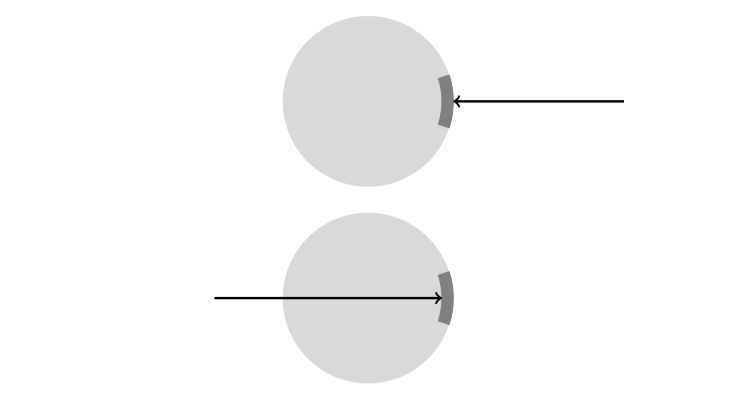
\includegraphics[width=\linewidth]{figures/incoming-outgoing}
  \caption{Angular flux impinged on an FSR from the moderator (top) and after traversing the fuel (bottom). \textit{Image courtesy of N. Gibson~\cite{gibson2016thesis}.}}
\label{fig:incoming-outgoing}
\end{figure}


\begin{figure}[h]
\begin{subfigure}{.45\textwidth}
  \centering
  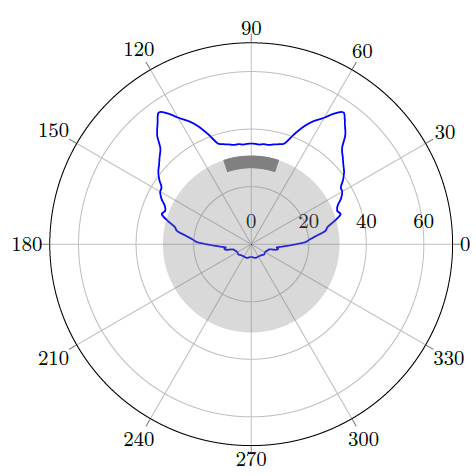
\includegraphics[width=0.9\linewidth]{figures/batman-1}
  \caption{}
  \label{fig:batman-plots-a}
\end{subfigure}
\begin{subfigure}{.45\textwidth}
  \centering
  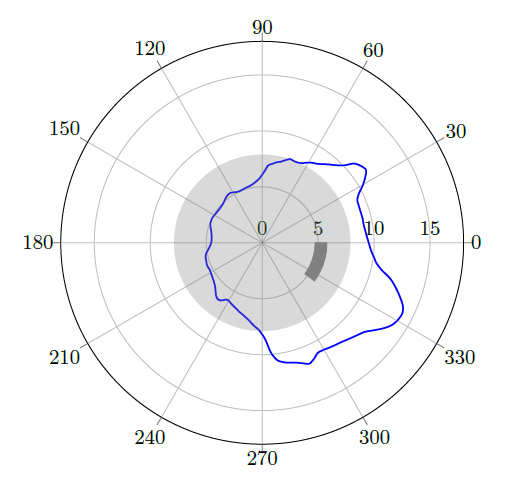
\includegraphics[width=0.9\linewidth]{figures/batman-2}
  \caption{}
  \label{fig:batman-plots-b}
\end{subfigure}
\caption{Angular-dependent capture MGXS for the 6.67 eV resonance group as a function of azimuthal angle for two different FSRs. The radial axis is given in units of barns and the azimuthal axis in units of degrees.}
\label{fig:batman-plots}
\end{figure}
